\chapter{Технологическая часть}

В данной части рассматривается выбор средств реализации, описывается структура классов программы и приводится интерфейс программного
обеспечения.

\section{Средства реализации}

Для реализации программного обеспечения выбран язык С++~\cite{cpp}. Выбор обусловлен скоростью выполнения и наличием опыта работы с ним, также язык представляет весь необходимый функционал для решения поставленной задачи и поддерживает объектно-ориентированную модель разработки.

Для реализации пользовательского интерфейса программного обеспечения выбран фреймворк $Qt$~\cite{qt}, который содержит в себе средства, позволяющие работать напрямую с пикселями.

Средой разработки был выбран $Qt Creator$~\cite{qt_creator}, который обладает всем необходимым функционалом для написания, отладки программ, и создания графического пользовательского интерфейса.

Для сборки программного обеспечения использовалась утилита $qmake$~\cite{qmake}.

\clearpage

\section{Структура классов}

Диаграмма классов представлена на рисунке~\ref{fig:uml}.

\begin{figure}[H]
    \centering
    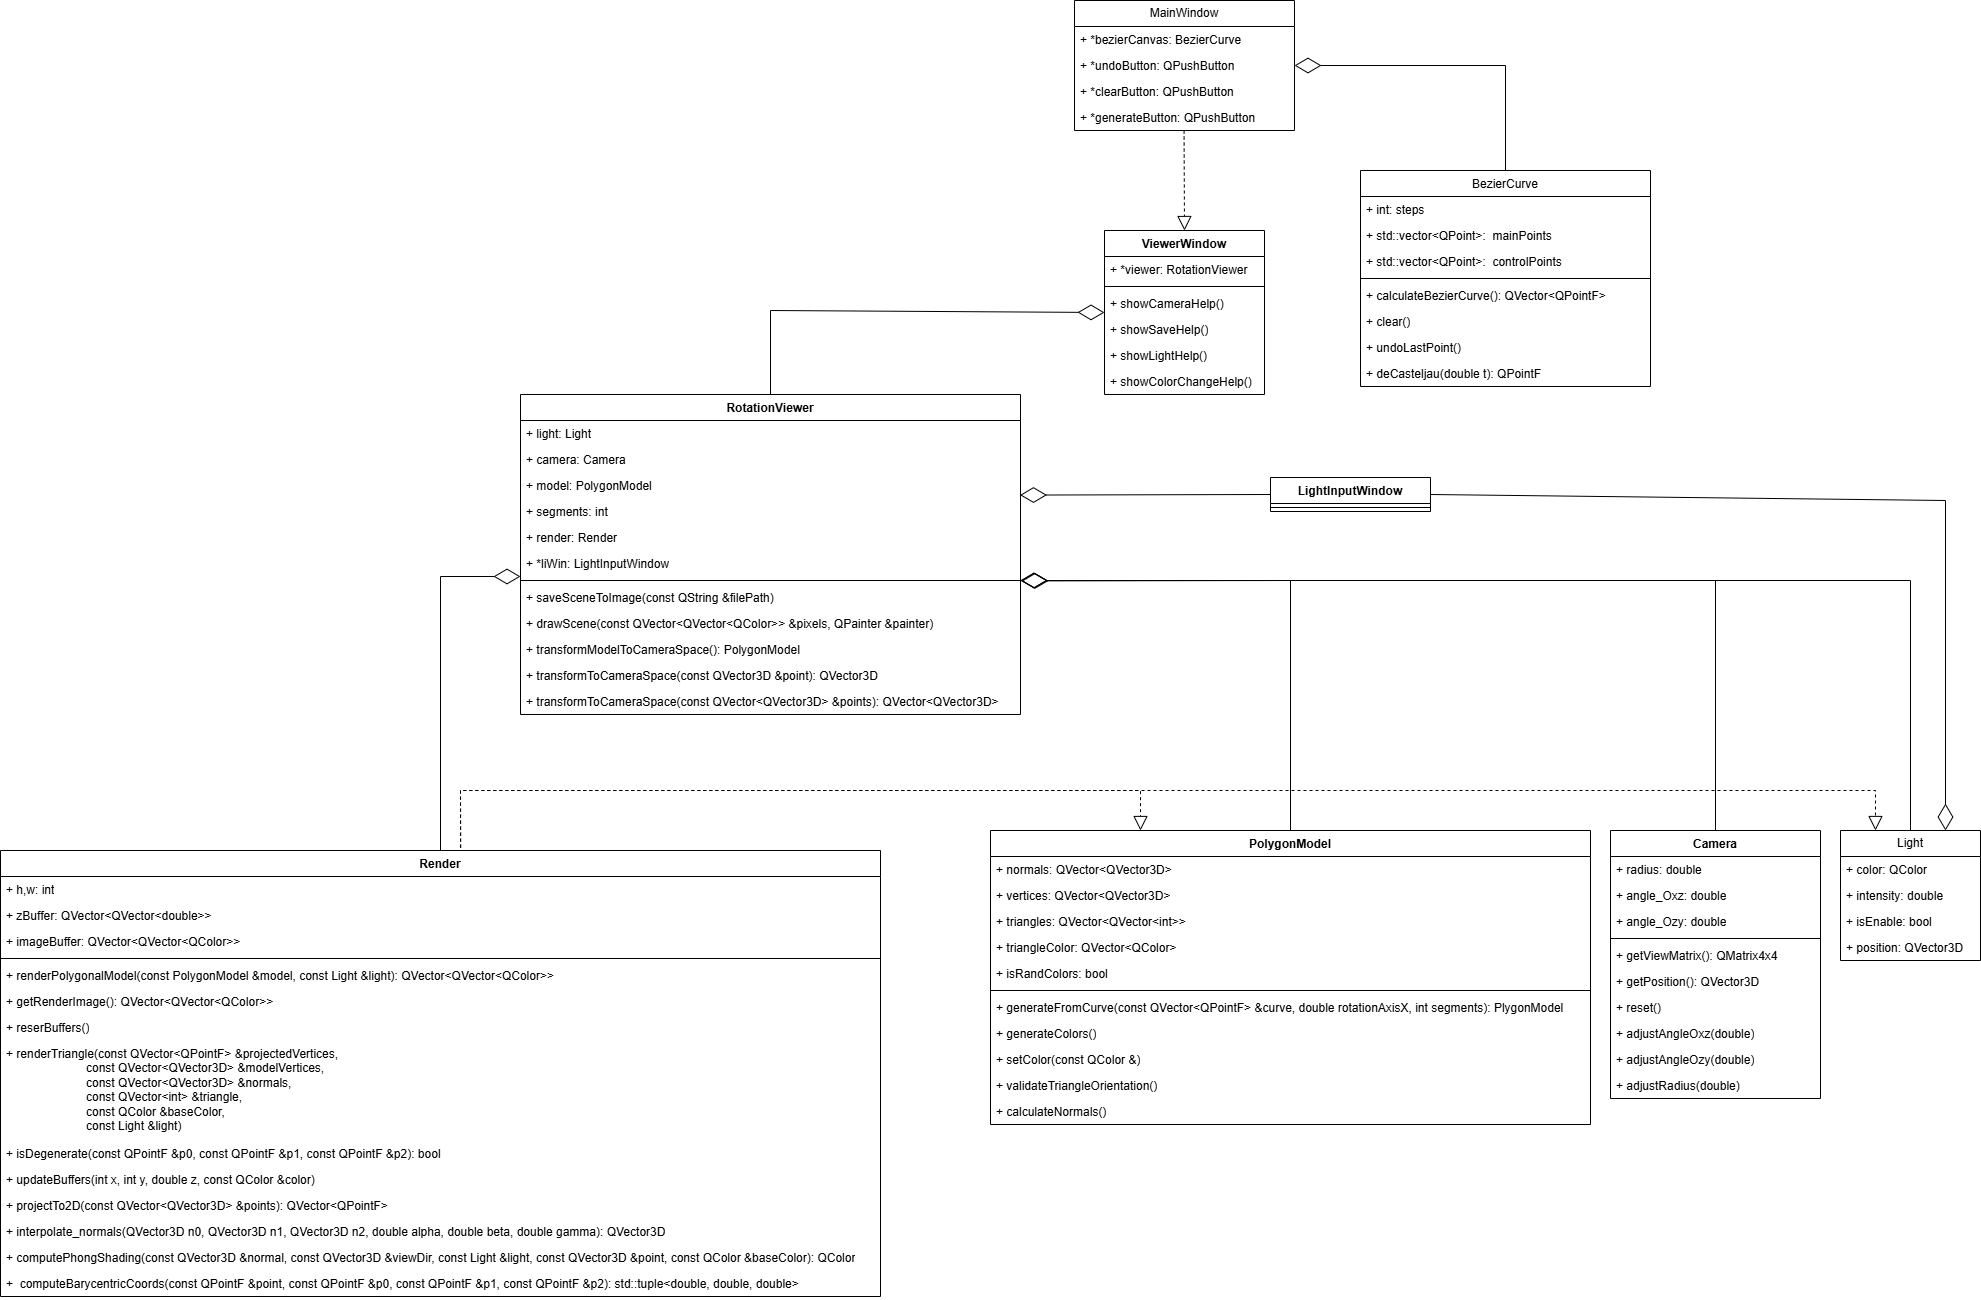
\includegraphics[width=1\linewidth]{images/diograms/uml.png}
    \caption{UML диаграмма классов}
    \label{fig:uml}
\end{figure}

\section{Интерфейс программного обеспечения}

Интерфейс программы представлен на рисунках~\ref{fig:interface1}~---~\ref{fig:interface6}.

\begin{figure}[H]
    \centering
    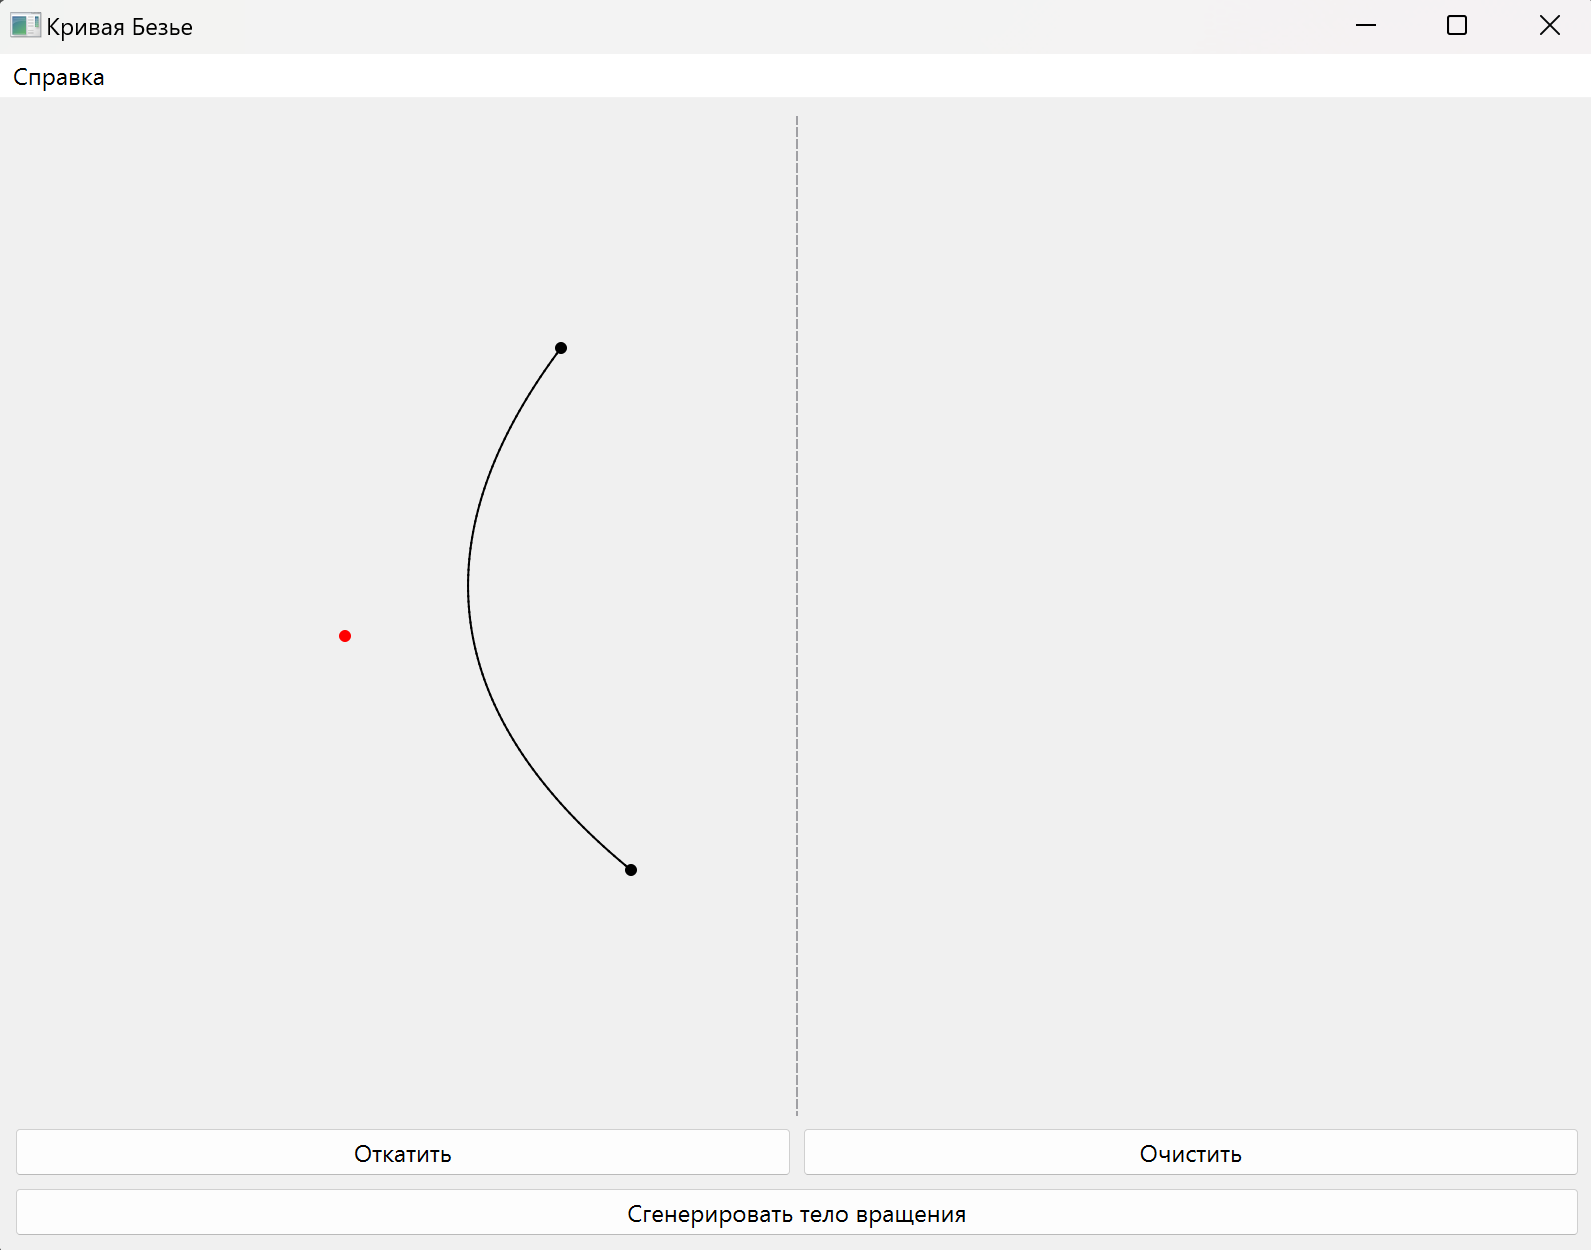
\includegraphics[width=0.8\linewidth]{images/interface/bezier.png}
    \caption{Окно ввода кривой Безье}
    \label{fig:interface1}
\end{figure}

\begin{figure}[H]
    \centering
    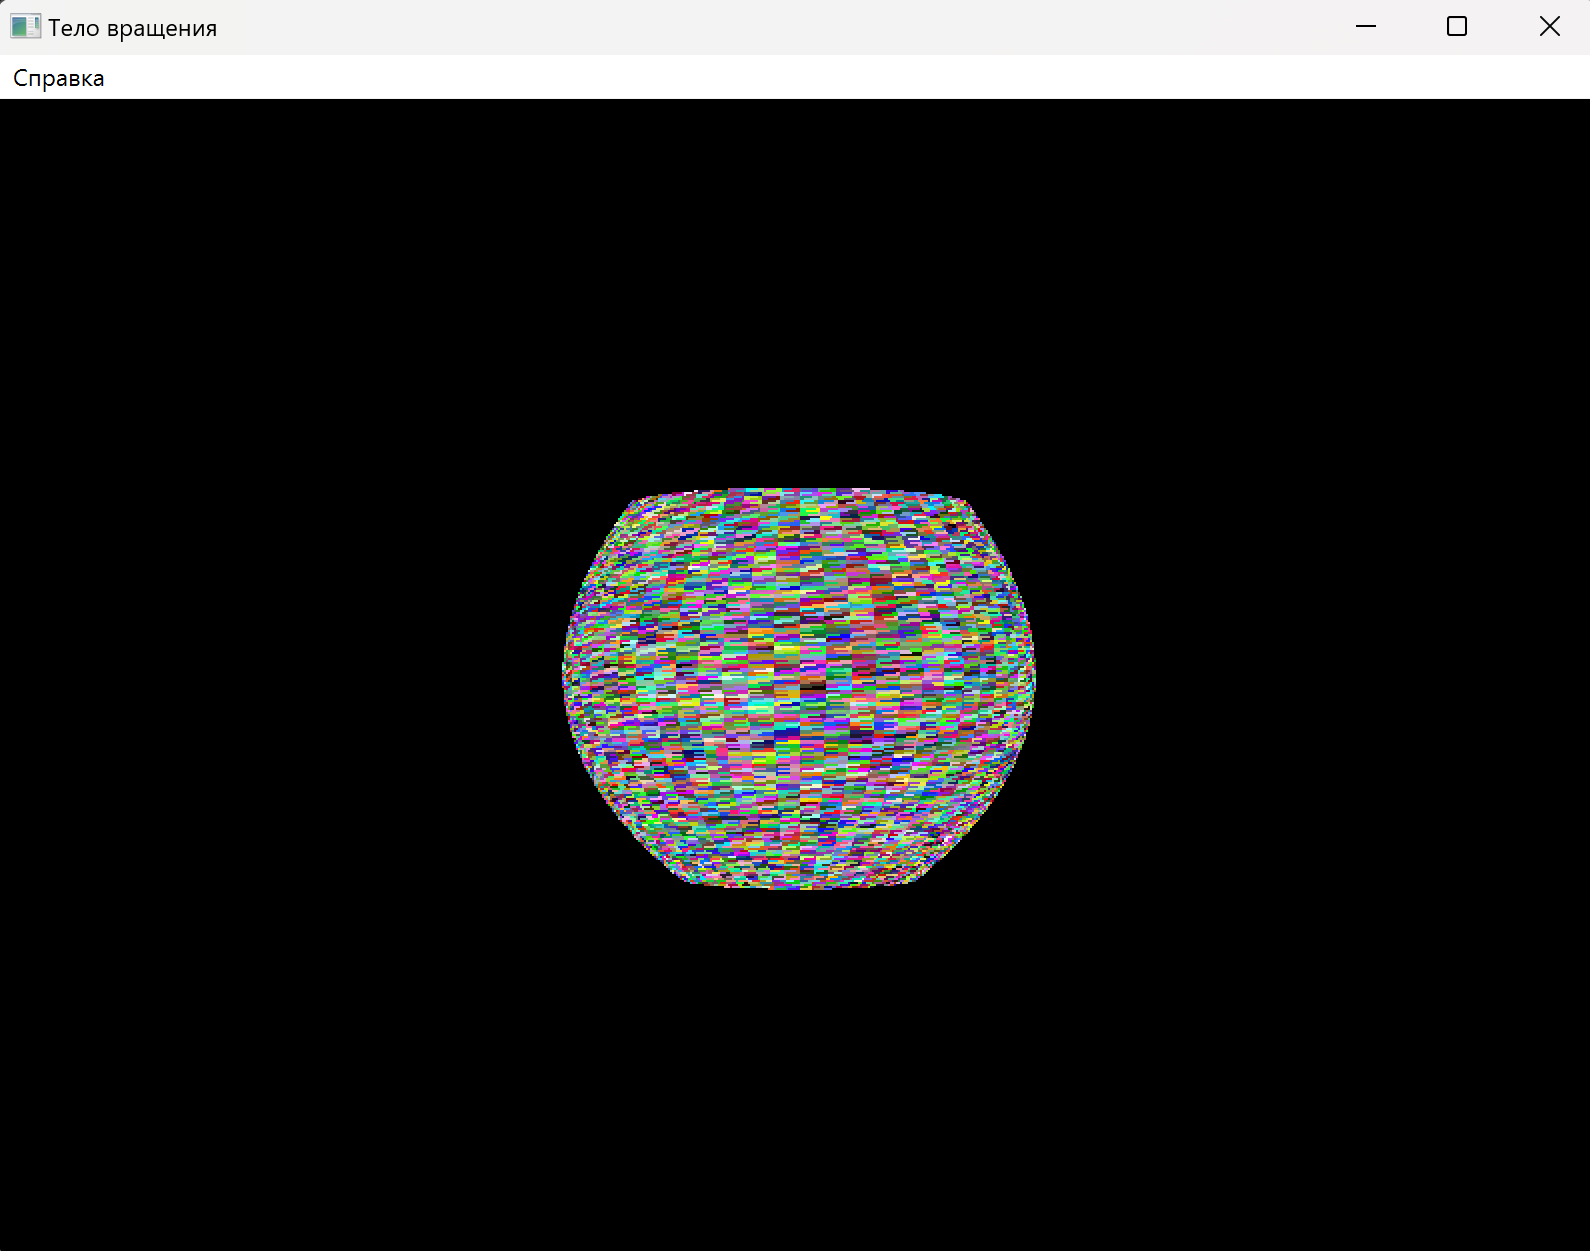
\includegraphics[width=0.8\linewidth]{images/interface/gen_body.png}
    \caption{Окно с телом вращения}
    \label{fig:interface2}
\end{figure}

\begin{figure}[H]
    \centering
    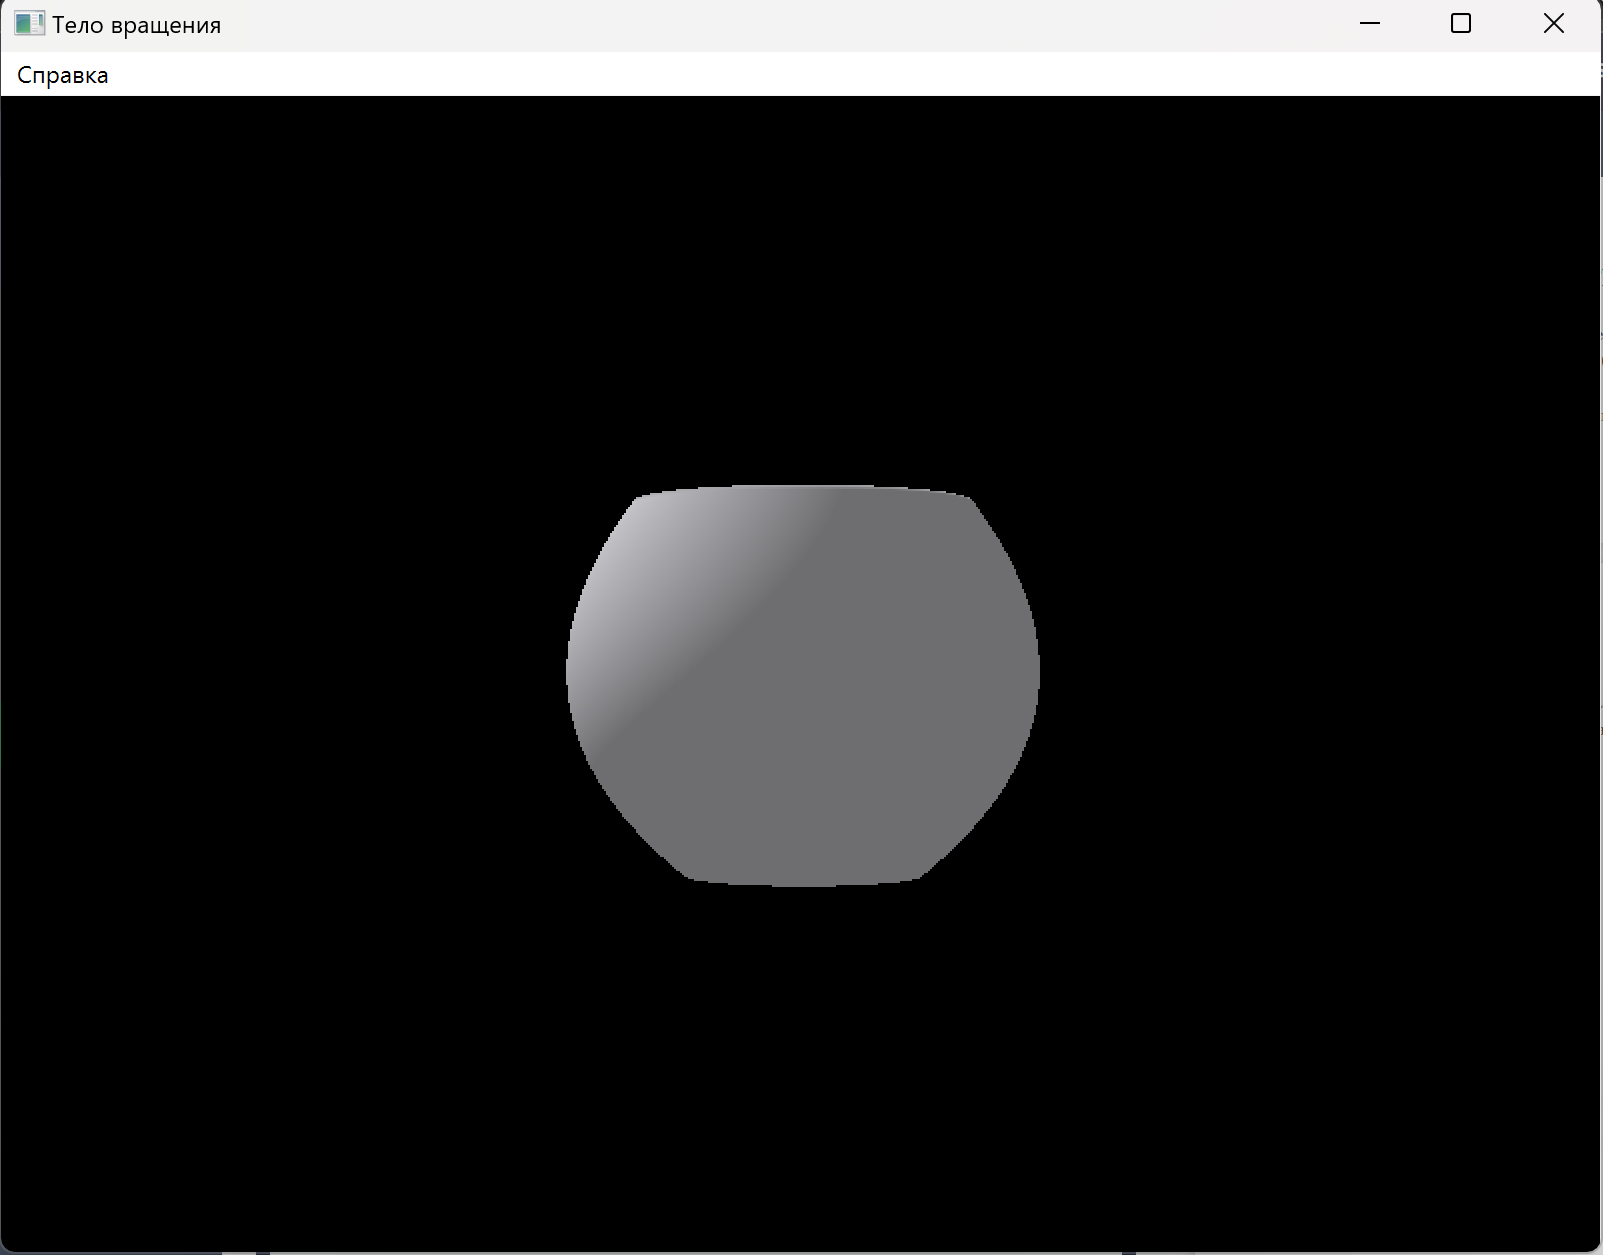
\includegraphics[width=0.8\linewidth]{images/interface/light_body.png}
    \caption{Окно с освещенным телом вращения}
    \label{fig:interface3}
\end{figure}

\begin{figure}[H]
    \centering
    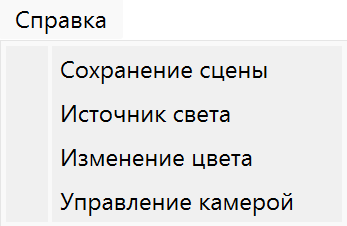
\includegraphics[width=0.8\linewidth]{images/interface/info.png}
    \caption{Справочная информация}
    \label{fig:interface4}
\end{figure}

\begin{figure}[H]
    \centering
    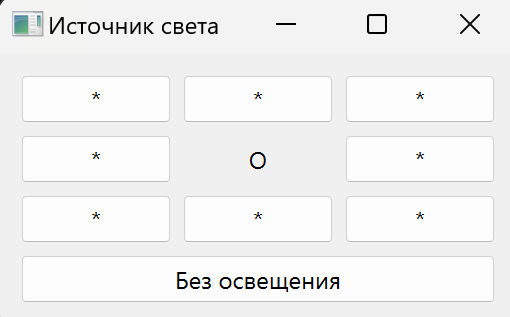
\includegraphics[width=0.8\linewidth]{images/interface/light_input.png}
    \caption{Ввод положения камеры}
    \label{fig:interface6}
\end{figure}
